\section{Molten Salt Fast Reactor}

The \gls{MSFR} is a reference design of a circulating-fuel \gls{MSR} developed
under the EURATOM \gls{EVOL} \cite{euratom_final_2015} and \gls{SAMOFAR}
\cite{kloosterman_20_2017} projects. The core of the
\gls{MSFR} consists of a 9 m$^3$ pool of fuel salt flowing upwards
\cite{serp_molten_2014}. At the top
of the core, the fuel salt flow separates into sixteen individual peripheral
loops, passing through the pumps, heat exchangers, and other instrumentation,
before flowing back into the active core region from the bottom. The core is
surrounded axially by nickel alloy reflectors, and radially by a toroidal
blanket tank containing fertile salt for
breeding. A layer of boron carbide absorber further protects the outer
components from excessive neutron damage. The main reactor specifications and
schematic view are shown in Table \ref{table:msfr} and Fig. \ref{fig:msfr}
respectively. 
%
\begin{table}[htb!]
	\caption{Main specifications of the \gls{MSFR} concept
				\cite{serp_molten_2014}.}
	\centering
	\begin{tabular}{ l r }
		\hline
		Parameter & Value \\
		\hline
		Thermal/Electric output [MW$_{\text{th}}$/MW$_{\text{e}}$] & 3000 /
		1500 
		\\
		Salt volume [m$^3$] & 18 \\
		Salt fraction in core & 0.5 \\
		Number of circulation loops & 16 \\
		Nominal flow rate [kg s$^{-1}$] & 18500  \\
		Nominal circulation time [s] & 4.0 \\
		Inlet/outlet temperature [K] & 923 / 1023 \\
		Blanket volume [m$^3$] & 7.3\\
		\hline
	\end{tabular}
	\label{table:msfr}
\end{table}
%
\begin{figure}[htb!] 
	\centering
	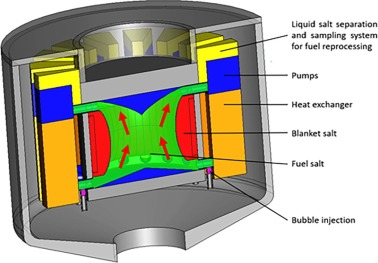
\includegraphics[width=0.6\textwidth]{MSFR}
	\caption{Schematic view of the MSFR concept \cite{serp_molten_2014}.}
	\label{fig:msfr}
\end{figure}

For the $^{232}$Th/$^{233}$U breeder configuration, the fuel and blanket salts
are composed of eutectic mixtures of 77.5\% LiF - 22.5\% AcF$_4$, where
AcF$_4$ represents actinide fluorides, uranium and thorium fluoride
\cite{serp_molten_2014}. A mole
fraction of approximately 1\% $^{233}$U is required for criticality; most
studies adjust the composition to achieve criticality at a uniform temperature
973 K as was done in the \gls{MSFR} neutronics benchmark paper
\cite{brovchenko_neutronic_2019}. Breeding ratios of up to 1.1 are expected
for the \gls{MSFR} \cite{fiorina_molten_2013}.

According to the design specifications, the inlet and outlet temperatures of
the fuel salt are to be 923 K and 1023 K respectively. This was motivated by
the desire for a 50 K minimum buffer between the operating temperatures
and the melting point of the salt \cite{euratom_final_2015}.
Having a secondary coolant loop adds a layer of containment between the
radioactive material and the outside environment. The exact specifications of
the heat exchanger and the secondary coolant loop are yet to be determined.
Thus, we assumed a secondary coolant temperature of 823 K with a heat transfer
coefficient value that corresponds to the intended 100 K temperature drop in
the fuel salt.
